A very often assumed scenario in the massive MIMO society was evaluated in this experiment, similar to the one-ring model \cite{bjornson2017massive}, where the BS located on top of a tall building while all UEs were on the far-field and surrounded by scatters. The scenario fits to the topic of pilot decontamination, as compared to the previous  non-line-of-sight (NLoS) measurement \cite{Chen2018pilot}, there is less overlapping in the angular support in this LoS scenario. If the angular support is not sparse, we can actually assume the channel property is closer to the non-correlated channel, and there is no benefit from pilot scheduling\footnote{Please refer to Fig. 3.5 in \cite{bjornson2017massive}, for the uncorrelated fading channel,  there is less impact in upper limit as compared to the correlated channel which overlaps in the angular domain. Moreover, it also shows no difference in pilot scheduling. However, the difference to theoretical one-ring model, from the measured angular transform in Section \ref{results}, the angular support is with irregular shape and spread. To differentiate angular information from different UEs is much more challenging in the measured LoS channel.}.   
\subsection{Outdoor LoS scenario}
An outdoor channel measurement was conducted in building ESAT2 of KU Leuven as presented in Fig. \ref{fig:The measured outdoor scenario}. The BS antenna arrays were located $21$m high from the ground and are constructed by patch antennas\cite{chen2017finite}, which were placed with a downtilt angle of $24^\circ$ in order to have a better main beam coverage for the UEs. Specifically, we deployed the antenna arrays in two different ways, i.e., collocated in the center as shown in green squares or distributed with a distance of $9.5$m as shown in yellow squares\footnote{The purpose of the two deployments is to collect different channel realizations.}. For each deployment of the BS arrays, we located a total of $36$ UEs on the ground. The $36$ UEs were equally divided into three rows. In each row, there were six two-by-two square meters grids. Note that at one time, we have only two UEs with antenna spacing of around $0.9\lambda$ located in the center of the grid. At each location, we collected $200$ OFDM symbols with a time spacing of $100ms$.
\subsection{Hardware and Software}

\begin{figure}[t!]
	\centering
	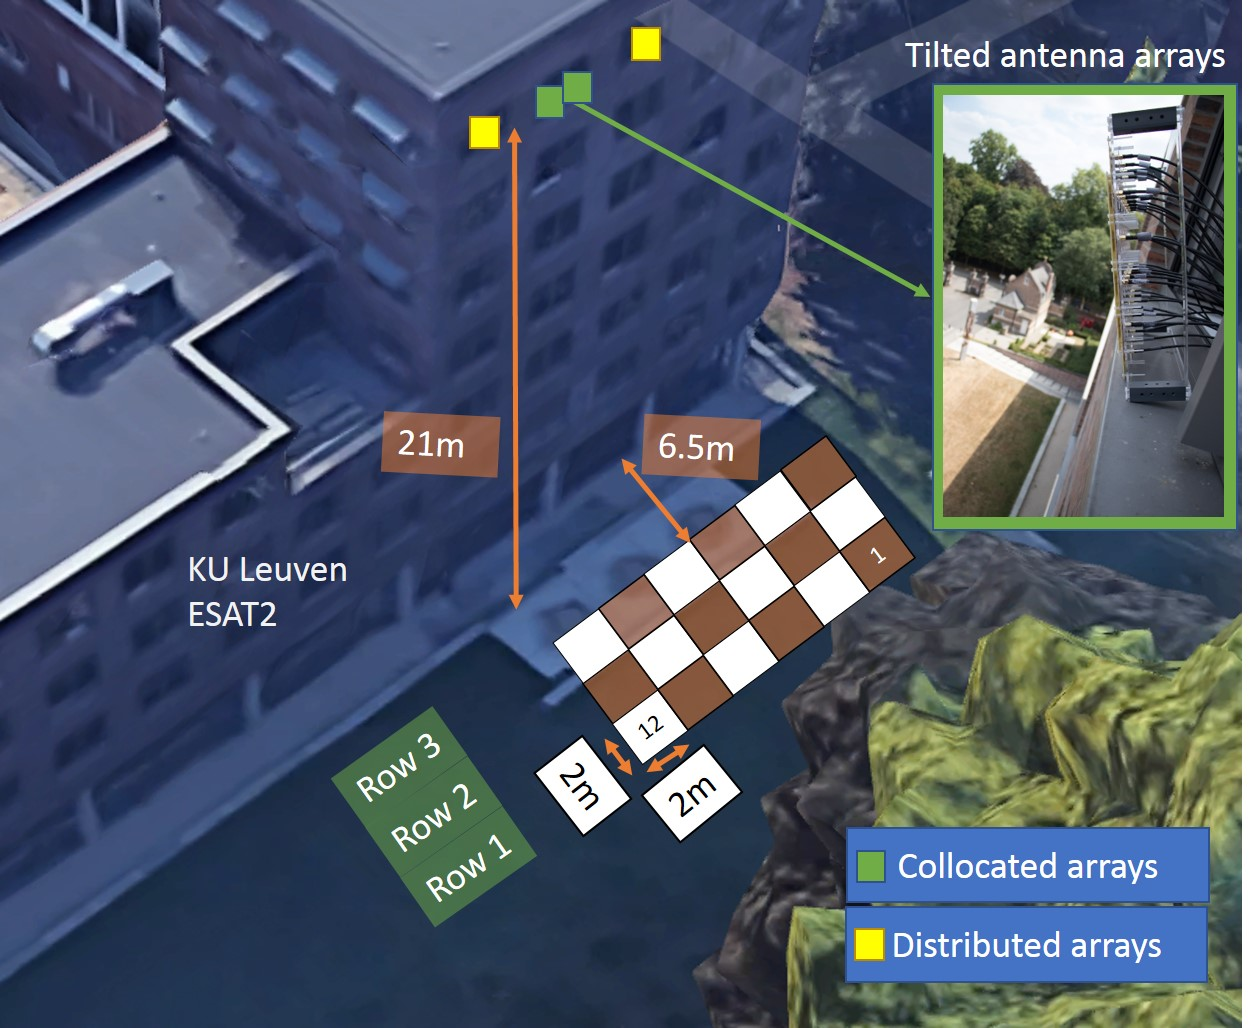
\includegraphics[width=1.0\linewidth]{figures/outdoor_scenario.jpg}
	\caption{We deployed $36$ UEs which were arranged into three rows in an outdoor LoS scenario. In each row, we put $12$ UEs, each pair of UEs are embedded in a single USRP with antenna spacing of $1.09\lambda$. Meanwhile, there were two ways of setting up the locations of the two-32 antennas patch arrays which were tilted in the front of windows for $24^\circ$ .}
	\label{fig:The measured outdoor scenario}
\end{figure}
\begin{figure}[t!]
	\centering
	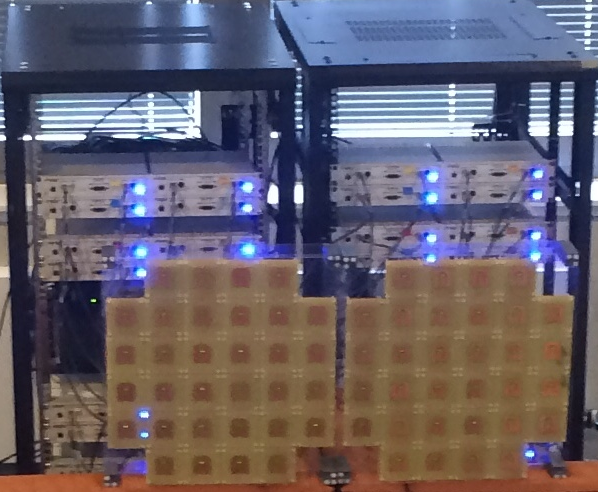
\includegraphics[width=1\linewidth]{figures/BSArrays.png}
	\caption{The KUL distributed massive MIMO testbed. There are two racks, each equips with $16$ USRPs for a total of $32$ RF chains. The two racks can be separated as far as $10$ meters because of the optical fibers that  are used for the back-haul connection.}
	\label{fig:BSArrays}
\end{figure}
\begin{figure}[t!]
	\centering
	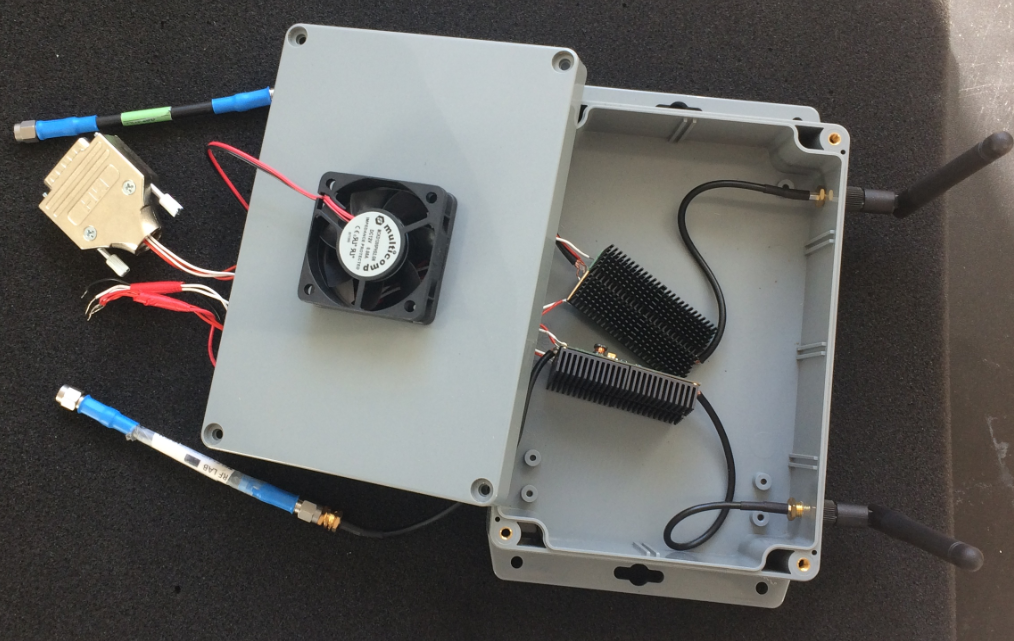
\includegraphics[width=1\linewidth]{figures/user_equipment.PNG}
	\caption{The user equipments were connected to off-the-shelf external-PAs in order to enlarge the sensitivity level for the long distance measurement. The antenna spacing is around $1.09\lambda$ for a center frequency of $2.61$GHz.}
	\label{fig:UserEquipment}
\end{figure}

\begin{figure}[t!]
	\centering
	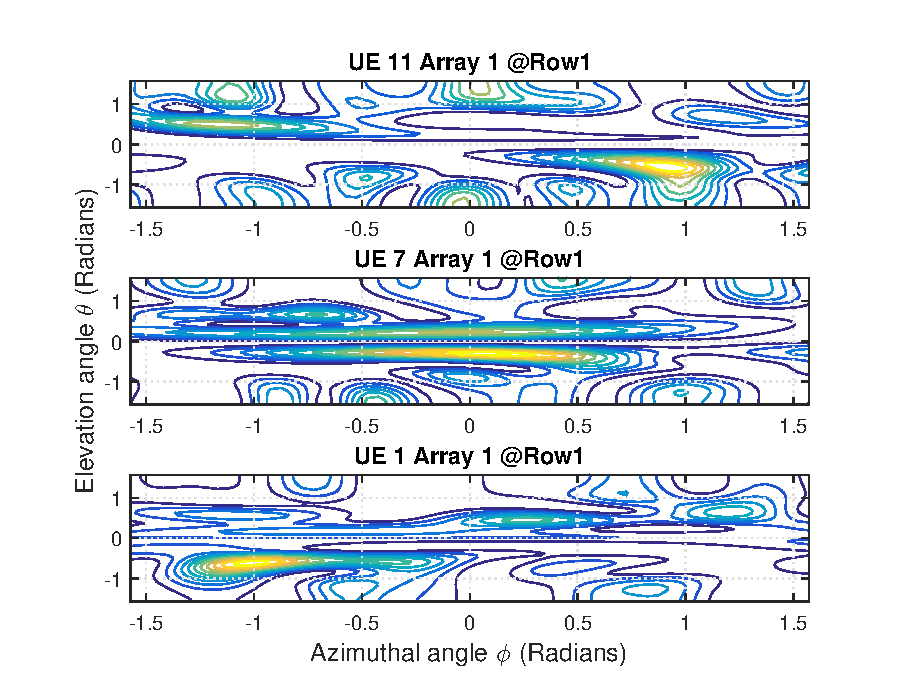
\includegraphics[width=1\linewidth]{figures/2DMUSICcollocated_row1_array1.eps}
	\caption{The 2D-MUSIC angular transformation of the measured outdoor channel. The related locations of the UEs are reflected in the angular domain.}
	\label{fig:2DMUSIC-measured-collocated-channel}
\end{figure}

\begin{figure}[t!]
	\centering
	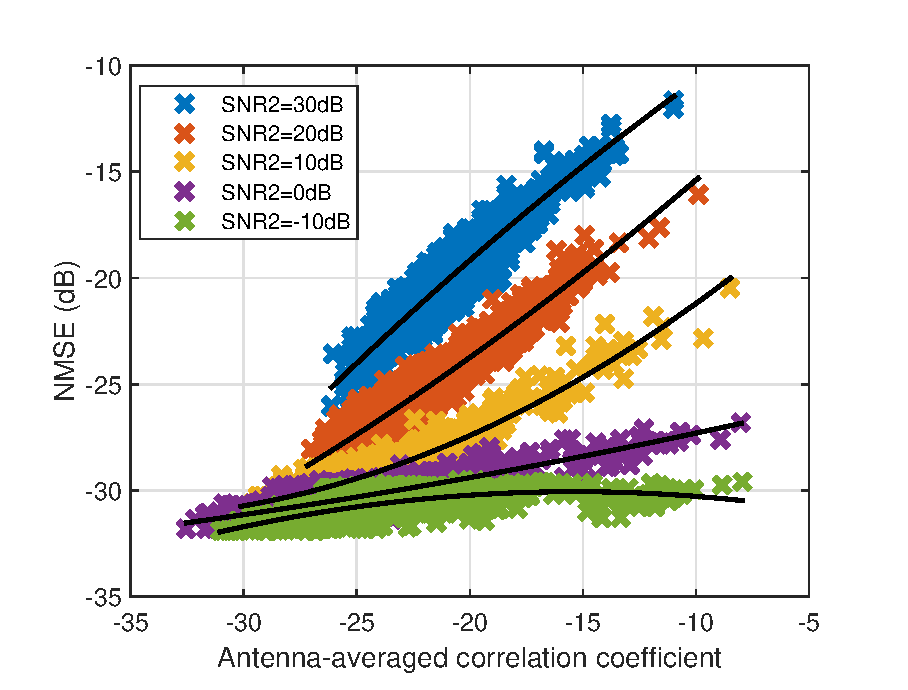
\includegraphics[width=1.0\linewidth]{figures/NMSE_correlation_allcases_collocated_wPA.eps}
	\caption{Correlation of NMSE channel estimation error to the antenna-averaged correlation coefficient. A spatially correlated channel, based on
the measured correlation channel.}
	\label{fig:channel_correlation_measured}
\end{figure}